\chapter{Introduction}


\section{The Size of a Cube}
\label{sec:size_of_a_cube}%

\todo[inline]{
  \footnotesize
  A picture of a cube (and a tetrahedron and dodecahedron).
  \\- What is the size of this cube?
  \\- Impossible to answer, since the picture only shows the abstract essence of a cube and not any physical cube in particular.
  \\- However, there are still ways to measure the cube as an abstraction.
  \\- A cube has 8 corners, 12 edges, and 6 faces.
  \\- In that sense, it is larger than a tetrahedron (picture) and smaller than a dodecahedron (picture).
  \\- Is any of these measures --- corners, edges, faces --- more fundamental than another?
  \\- This depends on what aspects of our object we are most interested in.
  \\- We may be interested in how many edges are between any two corners.
  \\- If we start at any corner, how many edges do we need to slide our finger across at most before we could reach any other corner?
  \\- In this context, we are really only interested in the connection structure, more than the geometrical object and a cube may as well be represented as in Figure~??.
  \\ A picture of a (planar) cubical graph (and a Wagner graph).
  \\- Having reduced our cube to a collection of dots and lines, we may notice an asymmetry between the number of each.
  \\- The number of dots can grow arbitrarily large without influencing the number of lines.
  \\- By contrast, the number of lines is bounded by approximately half the square of the number of dots.
  \\- \ldots
  \\- Introduce the Wagner graph.
  \\- This graph is not planar and hence it is not clear what its number of faces would be.
  \\- Still, it is very similar to the cubic graph.
  \\- Is it as large?
  \\- It has the same number of vertices (points) and edges (lines).
  \\- Other metrics are different, though.
  \\- Its diameter is 2, whereas that of the cube was 3.
  \\- We may envision actions on a graph that are easier on graphs with smaller diameter.
  \\- Does this make the diameter a good candidate for the size?
  \\- There are other structural properties, too, such as the size of a minimum vertex cover, and the chromatic number.
  \\- Both also differ from the cubical graph to the Wagner graph, the size of a minimum vertex cover being lower on the cubical graph, while the Wagner graph has a lower chromatic number.
  \\- \ldots
  \\- Where the size of a physical cube determines how large a pocket/box/hangar needs to be in order to contain the cube, the size of an abstract cube is determined by how long a description of its properties needs to be.
  \\- Example: description based on vertices (adjacency matrix) and on edges (edge list) --- which is shorter differs from the tetrahedron to the dodecahedron.
  \\- Some ways of describing a graph are more accommodating to answering a given question about a graph than others.
  \\- Amassing all possible ways to describe a graph (also, for instance, as a circuit for deciding edges), we obtain notion of size that is as good as any other.
  \\- Essentially, we have defined Kolmogorov complexity.
  \\- Careful counting reveals that whatever way to describe a graph we choose, there is a graph for which it is the best we can do (i.e.~a graph described by an incompressible string).
  \\- Therefore, no structural property is more `blessed' than any other.
  \\- It follows that the best way to describe a graph, and consequently the best way to measure its size, is dependent on what we want to do with the graph.
  \\- This is not only true of graphs but of any class of object we may consider to work with in a systematic way.
}


\section{Historical Encounters}

The word \emph{complexity} is used in various contexts and its meaning is not always made precise.
Still, it has often been observed that structural properties of data may influence the notion of complexity at hand.
In this thesis, we put forward a mathematical formalization of the notion of complexity, covering as many use cases as possible.
First, let us review some of the ways we may come across complexity and what structural properties these many forms of complexity are involved with.
In relation to their notions of complexity, each of these structural properties points at a line of thinking that is essentially parameterized.
In Chapter~\ref{ch:parameterizations}, this parameterized nature is made explicit by rephrasing the corresponding results in a unified parameterized framework.

\subsection{Computability}
Some sets are intrinsically undecidable.
For such sets, there is no effective procedure that is able to distinguish the members of the set from the nonmembers of the set.
This is a very extreme form of complexity:
We are unable to determine membership in undecidable sets uniformly not because we are perhaps not clever enough, but because it is fundamentally impossible.
Undecidable sets, however, are not all equally undecidable.
It is possible to organize many sets in a hierarchy of (un)decidability.
In fact, there are many ways to do so.

One hierarchy in which sets can be placed based on their decidability is the \defkey{arithmetical hierarchy}, due to \textcite{kleene1943recursive}.
This hierarchy consists of classes of sets that are defined inductively.
The classifications are denoted $\Sigma^0_n$ and $\Pi^0_n$, where $n$ is a natural number.
A set $S$ is in $\Sigma^0_{n+1}$ if there is a set $P$ in $\Pi^0_n$ such that we have
\begin{align*}
  S &= \{x \st \exists y\colon (x, y) \in P\}.
\intertext{
  Observe that the set $P$ is a set of pairs.
  Conversely, a set $P$ is in $\Pi^0_{n + 1}$ if there is a set of pairs $S$ in $\Sigma^0_n$ such that we have
}
  P &= \{x \st \forall y\colon (x, y) \in S\}.
\end{align*}
All that remains to define the arithmetical hierarchy is a definition of the base case, the classes $\Sigma^0_0$ and $\Pi^0_0$.
We follow \textcite{rogers1967theory} and \textcite{downey2010algorithmic} and set both classes equal to the class of decidable sets.
Originally, \citeauthor{kleene1943recursive} chose a smaller class, namely that of sets definable through `primitive recursive' predicates.
Yet another option is to take for $\Sigma^0_0$ and $\Pi^0_0$ the class of sets definable in first-order~logic with only bounded quantifiers \parencite{odifreddi1992classical}.
We shall not go into details about these alternatives.
Whichever definition we adhere to, we end up with the same classes $\Sigma^0_n$ and $\Pi^0_n$, whenever $n$ is at least $1$.
To wit, regardless of our choice for $\Sigma^0_0$ and $\Pi^0_0$, a set is in $\Sigma^0_1$ precisely when it is semidecidable (also known as \emph{recursively enumerable}) \parencite{kleene1943recursive,odifreddi1992classical,rogers1967theory}.
Likewise, the complement of a semidecidable set is in $\Pi^0_1$, as $\exists$ and $\forall$ are dual to each other in the sense that, for every predicate $Q$ we have
\begin{equation*}
  \lnot \exists x\colon Q(x) \:\iff\: \forall x\colon \lnot Q(x).
\end{equation*}
Indeed, a set $S$ is in $\Sigma^0_n$ if there is a decidable set $A$ such that we have
\begin{equation}
\label{eq:arithmetical_hierarchy}
  S = \{x \st \exists y_1\colon \forall y_2\colon\exists y_3\colon \ldots\colon ((\cdots((x, y_1), y_2)\ldots, y_{n-1}), y_n) \in A\}
\end{equation}
and similarly for $\Pi^0_n$ when we exchange $\exists$ and $\forall$.
It follows that, in general, a set is in $\Sigma^0_n$ if its complement is in $\Pi^0_n$.
As, for $n$ at least $1$, the classes $\Sigma^0_n$ and $\Pi^0_n$ are unequal, neither is closed with respect to taking complements.
For convenience, we therefore define classes $\Delta^0_n$ as the intersection of $\Sigma^0_n$ and $\Pi^0_n$.
These classes are closed with respect to taking complements.
Remark that sets in $\Delta^0_1$ are both semidecidable and have a semidecidable complement, and are therefore decidable.
Visually, the arithmetical hierarchy thus looks like depicted in Figure~\ref{fig:arithmetical_hierarchy}.
\begin{figure}
  \centering
  \begin{subfigure}{0.4\textwidth}
    \centering
    \begin{tikzpicture}
      \graph[layered layout, grow'=up, sibling distance=6em, edges={draw=none}, edge quotes={sloped, allow upside down}]{
        "$\Delta^0_0$" --["$=$"] {
          "$\Sigma^0_0$", "$\Pi^0_0$"
        } --["$=$"] "$\Delta^0_1$" ->["$\subset$"] {
          "$\Sigma^0_1$", "$\Pi^0_1$"
        } ->["$\subset$"] "$\Delta^0_2$" ->["$\subset$"] {
          "$\Sigma^0_2$", "$\Pi^0_2$"
        } ->["$\subset$"] "\vdots"
      };
    \end{tikzpicture}
    \caption{
      The arithmetical hierarchy.
      \\\hspace{0pt} \\\hspace{0pt} % For alignment
    }
    \label{fig:arithmetical_hierarchy}
  \end{subfigure}
  \qquad
  \begin{subfigure}{0.4\textwidth}
    \centering
    \begin{tikzpicture}
      \graph[layered layout, grow'=up, sibling distance=6em, edges={draw=none}, edge quotes={sloped, allow upside down}]{
        "$\Delta^{-1}_1\mathrlap{\:= \Delta^0_1}$" ->["$\subset$"] {
          "$\mathllap{\Sigma^0_1 =\:}\Sigma^{-1}_1$", "$\Pi^{-1}_1\mathrlap{\:= \Pi^0_1}$"
        } ->["$\subset$"] "$\Delta^{-1}_2$" ->["$\subset$"] {
          "$\Sigma^{-1}_2$", "$\Pi^{-1}_2$"
        } ->["$\subset$"] "$\Delta^{-1}_3$" ->["$\subset$"] {
          "$\Sigma^{-1}_3$", "$\Pi^{-1}_3$"
        } ->["$\subset$"] "\vdots"
      };
    \end{tikzpicture}
    \caption{
      The difference hierarchy lies below the $\Delta^0_2$ level of the arithmetical hierarchy.
    }
    \label{fig:difference_hierarchy}
  \end{subfigure}
  \caption{
    The arithmetical hierarchy and the difference hierarchy are both infinite hierarchies of classes of sets.
  }
\end{figure}

Returning to undecidability as a form of complexity, the arithmetical hierarchy provides a means to analyze complexity.
For sets that appear in one of the classes of the arithmetical hierarchy, say $\Delta^0_n$, we may assign the level at which it occurs, $n$, to the complexity of the set.
Thus, we can compare how undecidable certain sets are.
As demonstrated by~\eqref{eq:arithmetical_hierarchy}, this notion of complexity ties in with a more or less structural property of the set it applies to.
The number of quantifier alternations required for defining a set starting from a decidable set expresses its complexity.

At a conceptual level, one of the focal points of computability theory is the behavior of computations in the limit.
Computations that terminate eventually are said to converge, and computations that never terminate are said to diverge.
From this perspective, it is clear how the sets in $\Sigma^0_1$, the semidecidable sets, are slightly more complex then the decidable sets.
Decidable sets have decision procedures and those procedures converge on all inputs.
For semidecidable sets on the other hand, convergence of a procedure that tries to determine membership can only be guaranteed on the members of the set.
Ascending further in the arithmetical hierarchy, it becomes near-impossible to give characterisations of the sets in terms of convergence.
This is one reason to look for measures of complexity-beyond-decidability that increase complexity more gradually.
One such measure was introduced by \textcite{ershov1968hierarchyi} some 25 years after the introduction of the arithmetical hierarchy.
This measure also revolves around a hierarchy of classes of sets and is in that regard similar in spirit to the arithmetical hierarchy.
We have seen that the $\Sigma$ and $\Pi$ classes of the arithmetical hierarchy are not closed with respect to taking complements.
The starting point of \citeauthor{ershov1968hierarchyi}'s hierarchy was the observation that these classes are also not closed with respect to taking relative complements.
Given two sets $A$ and $B$ in some class $\Sigma^0_n$, with $n$ at least $1$, the set $A \setminus B$ need not be in $\Sigma^0_n$ and similarly for the classes $\Pi^0_n$.
However, when $A$ and $B$ are taken from $\Sigma^0_n$, we may go about deciding whether a given $x$ is in $A \setminus B$ as follows.
\begin{codelisting}
\item
  We assume $x$ is neither in $A$ nor in $B$ and if our computations are interrupted and we are asked our best guess about $x$, we answer that it \emph{is not} in $A \setminus B$.
\item
  We try to find out whether $x$ is in $A$ by running a procedure that halts precisely on the members of $A$.
  If this procedure halts, we have learned that $x$ is in $A$.
  In case we are then asked our best guess about $x$, we answer that it \emph{is} in $A \setminus B$.
\item
  Having found that $x$ is in $A$, we try to find out whether $x$ is in $B$ by running a procedure that halts precisely on the members of $B$.
  If this procedure halts, we have learned that $x$ is also in $B$.
  In case we are later asked our best guess about $x$, we answer that it \emph{is not} in $A \setminus B$.
\end{codelisting}
Only in the final situation, we can answer a membership query with centainty.
Therefore, our procedure should be considered a kind of approximation of a decision procedure.
Observe that the procedure adjusts its knowledge about membership of $x$ in $A \setminus B$ at most twice.
Procedures that are not convergent in the classical sense, but are allowed to `change their mind' a finite number of times were first put forward by \textcite{putnam1965trial} and \textcite{gold1965limiting}.

The idea of \citeauthor{ershov1968hierarchyi} was to base a hierarchy on number of times a decision procedure in the sense of \citeauthor{putnam1965trial} and \citeauthor{gold1965limiting} is allowed to change its mind.
The resulting hierarchy is known today as the \defkey{difference hierarchy} \parencite{downey2010algorithmic}.
The classes of the difference hierarchy are denoted $\Sigma^{-1}_n$ and $\Pi^{-1}_n$.
For sets $A, B$, let $A \symdiff B$ denote the symmetric difference $(A \setminus B) \cup (B \setminus A)$.
A set $S$ is in $\Sigma^{-1}_n$ if there are sets $A_1, A_2, A_3, \ldots A_n$ in $\Sigma^0_1$ such that we have
\begin{equation}
\label{eq:difference_hierarchy}
  S = A_1 \symdiff A_2 \symdiff A_3 \symdiff \ldots \symdiff A_n.
\end{equation}
Like in the arithmetical hierarchy, a set $P$ is in $\Pi^{-1}_n$ if its complement, $P^\complement$ is in $\Sigma^{-1}_n$.
Note that when $n$ is odd, we have
\begin{equation*}
  (A_1 \symdiff A_2 \symdiff A_3 \symdiff \ldots \symdiff A_n)^\complement = A_1^\complement \symdiff A_2^\complement \symdiff A_3^\complement \symdiff \ldots \symdiff A_n^\complement.
\end{equation*}
Therefore, for odd $n$, a set $P$ is in $\Pi^{-1}_n$ if there are sets $A_1, A_2, A_3, \ldots A_n$ in $\Pi^0_1$ such that we have
\begin{equation*}
  P = A_1 \symdiff A_2 \symdiff A_3 \symdiff \ldots \symdiff A_n.
\end{equation*}
These definitions are equivalent to the original characterization by \textcite{ershov1968hierarchyi} that was stated in terms of unions of disjoint relative complements.
The equivalence follows from elementary identities.
The resulting hierarchy, including the levels $\Delta^{-1}_n$ that are the intersection of $\Sigma^{-1}_n$ and $\Pi^{-1}_n$, is depicted in Figure~\ref{fig:difference_hierarchy}.

Because the $\Delta^0_2$ class is closed under taking unions, intersections, and complements, it is also closed under taking symmetric differences.
Moreover, it includes both $\Sigma^0_1$ and $\Pi^0_1$, thus for all natural numbers $n$, the classes $\Sigma^{-1}_n$, $\Pi^{-1}_n$, and $\Delta^{-1}_n$ of the difference hierarchy are included in $\Delta^0_2$.
Consequently, the difference hierarchy is only relevant for sets that are not too complicated according to the arithmetical hierarchy.
Still, its core ideas make the ensuing notion of complexity an interesting measure of undecidability.
As we have seen, the number of semidecidable sets needed to write a set like in~\eqref{eq:difference_hierarchy} relates to a generalized form of convergence of computation.

\subsection{Computational Tractability}
In computational complexity theory, a set is deemed complex if it is intractable.
Here, tractability is customarily taken with respect to the running time behavior of decision procedures.
While we can measure the time a decision procedure takes on a specific input, we are primarily interested in the way this time scales to other, unknown, inputs.
The running time of a decision procedure is therefore traditionally measured as a function of, or functional behavior relative to, the size of its input.
As we saw in Section~\ref{sec:size_of_a_cube}, the notion of input size is heavily reliant on the choice of an encoding scheme for inputs.
No computable encoding scheme reflects all possible structural aspects an input may have.
This is especially visible in contexts that offer some `standard' encoding.
For instance, in graph theory, graphs are often thought of as encoded by an adjacency matrix.
In that case, the size of a graph is determined by the number of its vertices.
However, in deciding a set of graphs, certain structural properties other than the number of vertices may be exploitable by a decision procedure.
Regarding sets that are intractable because the running time of a decision procedure is at least exponential as a function of the input size, \citeauthor{garey1979computers} remark the following.
\blockcquote{garey1979computers}{
  \textelp{} there are a variety of ways in which the time complexity of an algorithm can be \enquote{exponential,} some of which might be preferable to others.
  This is especially evident when, as is customary in practice, we consider time complexity expressed in terms of natural problem parameters instead of the artificially constructed \enquote{input length.}
}
When restricting to inputs on which such \emph{natural parameters} assume small values, a set that is initially intractable may indeed become tractable.
As inputs with low parameter values may be abundant, it may be that large subsets of the input space are easy to digest for some decision procedure.
In addition, \citeauthor{garey1979computers} note that inputs encountered in practice may tend to have low parameter values:
\enquote{\textelp{} in practice it is often the subproblem, rather than the general problem, that we are called upon to solve.}

\begin{example}
  We can model a social network by a graph, representing persons by vertices and connecting two vertices when the persons they represent know each other.
  Given a graph that models mutual acquaintance, we may ask how large a subset of people there exists that all know each other.
  This is formalized by the set
  \begin{align*}
    \pr{Clique} \deq \{(G, l) \st &\text{there is a set of at least $l$ vertices of the graph $G$} \\
    	&\text{that are pairwise connected}\}.
  \end{align*}

  Let $G$ be a graph with $n$ vertices and let $l$ be at most $n$.
  The number of possible subsets of the vertices of $G$ that are of size $l$ cannot be bounded by a polynomial of $n$ alone.
  In fact, when $l$ is approximately $\frac{n}{2}$, the number of subsets is exponential as a function of $n$.
  It is widely believed that there are no decision procedures for \pr{Clique} that have a subexponential running time.
  Nonetheless, given a subset of vertices of $G$, we can check whether its members are pairwise connected within a polynomial running time.

  However, this analysis disregards some practicalities that result from the situation we are modeling.
  It is rare to come across a person with very many mutual acquaintances.
  Therefore, it is safe to assume that in any graph we encounter as the model of a social network, no vertex is connected to more than, say, $20$ others.
  As a consequence, we find that in any graph encountered in practice, a set of pairwise connected vertices, a \emph{clique}, can contain at most $21$ elements.
  This means that the number of subsets of vertices that needs to be checked is less than $n^{21}$, which, as \citeauthor{garey1979computers} observe, is polynomial in $n$.
  While this already brings the running time down to polynomial, we shall see in Section~\ref{sec:parameterized_complexity_theory}, that a far more efficient decision procedure is not hard to come by.
\end{example}

The takeaway is that computational complexity is preferably measured by parameters of the input instead of by the input length alone.
Somehow, we need to decide which parameters to take into account.
Different decision procedures may favor different parameters.
Note, though, that it is possible to combine the benefits that different parameters may provide through aggregating multiple decision procedures.

\begin{example}
  One way to decide membership in \pr{Clique} is by generating an exhaustive list of candidate sets of vertices and checking whether any is a clique of the desired size.
  Suppose we want to decide whether a given graph $G$ has a clique of $l$ elements.
  The simplest implementation of the aforementioned design pattern starts out by generating all possible sets of $l$ vertices of $G$.
  However, other approaches are possible too.

  Suppose $l$ is even and we have a clique $(v_1, v_2, v_3, \ldots, v_l)$.
  Because these vertices form a clique there is, for $i \le \frac{l}{2}$, an edge connecting $v_i$ to $v_{i + 1}$ in $G$.
  Thus an alternative way to generate candidate sets of vertices is via all possible sets of $\frac{l}{2}$ edges, by taking the endpoints of the selected edges.
  Any clique of size $l$ is guaranteed to be generated this way.

  We can compare these two approaches by counting the number of candidate sets they consider.
  Let $n$ be the number of vertices in $G$ and $m$ the number of its edges.
  There are $\binom{n}{l}$ sets of $l$ vertices and $\binom{m}{l / 2}$ sets of $\frac{l}{2}$ edges.
  When either of these numbers is much smaller than the other, we expect the corresponding decision procedure to run much than the other.
  Thus, it pays to construct an aggregate decision procedure.
  This decision procedure would first compute both numbers and then run the decision procedure that is expected to be the fastest.

  The computational complexity of the vertex-centric decision procedure is best expressed as a function of the parameters $n$ and $l$.
  On the other hand, the complexity of the edge-centric decision procedure is best expressed as a function of the parameters $m$ and $l$.
  Our aggregate decision procedure demonstrates that it pays off to take into account multiple parameters.
  By we get a more detailed insight into the computational complexity of a set by taking into account more parameters.
  For some instances of \pr{Clique}, the running time bound available in terms of $n$ and $l$ is better than that in terms of $m$ and $l$ and vice versa.
\end{example}

The algorithm we presented for our aggregate decision procedure for \pr{Clique} in the example above combines two other algorithms.
Such algorithms are known as \emph{hybrid algorithms} \parencite{malek1994hybrid}.
They offer a best-of-both-worlds alternative in situations where we have two algorithms without one being better than the other.
From a parameterized point of view, hybrid algorithms combine the information of multiple input parameters and as such show how these parameters can interact.
This is relevant not only when we use parameters to measure computational complexity, but also in the design of ever faster polynomial-time algorithms.

\begin{example}
  \indexkey{example!sorting algorithms}%
  As a showcase of hybrid algorithms in the absence of computational complexity, we shall take a look at sorting algorithms.
  Even naive sorting algorithms, such as repeatedly finding the least value, manage to have a running time bounded by a polynomial of the length of the input list.
  Because sorting is such a common operation in algorithmics, extensive research has been put into the development of fast sorting algorithms.

  The quicksort algorithm \parencite{cormen2009introduction} makes a number of comparisons that is at most quadratic as a function of the length, $n$, of the input list.
  However, worst-case inputs are very rare and on average the algorithm needs roughly $n \log n$ comparisons.
  With in the order of $n \log n$ comparisons in the worst case, the heapsort algorithm \parencite{cormen2009introduction} appears at least as good as quicksort.
  Nevertheless, it has a higher overhead and in practice it is often outperformed by quicksort.
  By combining both algorithms, we can construct a sorting algorithm that is about as fast as quicksort, yet has a worst-case running time in the order of $n \log n$.
  This hybrid algorithm is known as \emph{introsort} \parencite{musser1997introspective} and is used by some prominent implementations of the \Cpp{} standard library.

  The way introsort chooses between its constituent algorithms, quicksort and heapsort, is not as up-front as it was in our hybrid decision procedure for \pr{Clique}.
  This matters when we want to identify parameters that express structure favored by either of the constituent algorithms.
  Instead of handing over the input to either quicksort or heapsort, the hybrid introsort hooks into the divide~and~conquer nature of quicksort.
  The core of the quicksort algorithm is that it splits its input list into a list of low values and a list of high values.
  These sublists can be sorted independently and for that, quicksort recursively invokes itself.
  Because the splitting stage requires some $n$ comparisons for a list of $n$ elements, we do not want the recursion depth to exceed a constant multiple of $\log n$.
  In the worst case, however, quicksort reaches a recursion depth of $n$.
  To mitigate this worst case behavior, introsort uses heapsort to sort the sublists when the recursion depth gets too high, say higher than $2 \log n$.
  Thus, we have found that the recursion depth reached by quicksort functions as a parameter of the input list.
  This parameter may appear somewhat unnatural and its specific value for a given list depends on the implementation of quicksort.
  For all implementations, however, input lists that get high parameter values can be constructed \parencite{mcilroy1999killer}.

  For short lists, insertion~sort \parencite{cormen2009introduction} is faster still than quicksort and heapsort.
  However, it makes a quadratic number of comparisons in the average case.
  Therefore it is suboptimal for all inputs of a length exceeding some platform-dependent constant.
  Many implementations of introsort use insertion~sort when the input list is short.
  Here, the parameter at play is evident.
  It is the length of the input list.

  The architecture of introsort follows quicksort and only for the base case of the recursion it deviates from that.
  In this way, introsort is based on an algorithm that has a bad worst-case running time, but is  fast in practice.
  Another hybrid sorting algorithm, timsort \parencite{peters:timsort}, takes the opposite approach.
  This algorithm was developed for for the Python programming language and is also used in the Java virtual machine and in the standard library of the Rust programming language.
  It is adapted from mergesort \parencite{cormen2009introduction}, which has a good worst-case running time, but fails to exploit patterns encountered in practice.
  Like quicksort, mergesort is a divide~and~conquer algorithm.
  Where introsort followed quicksort top-down and resorted to heapsort at high recursion depths, timsort follows a bottom-up implementation of mergesort.
  It uses insertion~sort to quickly prepare a base case that is as accommodating to mergesort as possible.
  Using insertion~sort for the base case is efficient, because insertion~sort is fast on short lists.
  The base case is prepared in such a way that the use of locally sorted parts of the input list is maximized.
  This makes timsort an \emph{adaptive} sorting algorithm.
  A proper analysis of timsort is therefore not possible on the basis of only the length of the input list as a parameter.
  In addition, it requires a parameter related to the locality of the disorder in the input list.
\end{example}

Note that a detailed analysis of the computational complexity of an algorithm may expose many parameters that influence the running time of the algorithm.
These parameters need not be independent of one another and their interactions need not be straightforward.
Parameterized computational complexity theorists are tasked with gaining insight in these interactions.

\subsection{Algorithmic Complexity}
Complexity, in whatever incarnation, can often be traced back to a lack of structure.
Highly structured objects are easy to analyze and an unlikely cause of complexity.
But what makes an object structured?
One answer could be \enquote{if it has many properties}, but this simply makes us wonder what counts as a property of an object.
Certainly, we want the properties of an object to tell us something about the object.
In other words, it must be special for an object to have a given property.
We mean this in a technical sense and assert that structural properties help in giving short descriptions of objects.

\begin{example}
  Consider graphs on $8$~vertices.
  There are
  \begin{align*}
    2^{\binom{8}{2}} &= \num{268435456}
  \intertext{
    such graphs.
    However, if we know that a particular graph has $9$~edges, we are left with only
  }
    \binom{\binom{8}{2}}{9} &= \phantom{00}\num{6906900}
  \end{align*}
  options.
  Because this is a substantial reduction, we can give a succinct description of a graph with $8$~vertices and $9$~edges by first giving its number of edges.

  The critical observer will have noticed that we have assumed a number of vertices that was fixed and known.
  Indeed, having $8$~vertices is in itself already a structural property of a graph.
  Without knowing the number of vertices in a graph that is being described to us, we have an infinite number of candidates to choose from.
\end{example}

Often, we can identify a value inside a structural property that can be generalized over.
The property can then be seen as an instantiation of an underlying property schema.
This is most apparent when the structural property has an element of counting in it, such as is the case with our \enquote{has $9$~edges} property in the example above.
\begin{example}[continued]
  Replacing the value~$9$ in the property \enquote{has $9$~edges} by the variable $e$, we obtain the property schema \enquote{has $e$~edges}.
\end{example}

Seldomly is it necessary to make a distinction between properties and property schemata.
However, it is useful here because it clarifies the relation between parameters, as encountered earlier, and properties.
Technically, parameters correspond to property schemata.

When working with description methods, it is necessary to settle, beforehand, what counts as a reasonable description method.
Were we to allow all possible mappings of objects to strings, we run into paradoxes like the Berry paradox \parencite[see][]{li2008introduction}.
This paradox shows that if any mapping goes, any object could be described in arbitrarily few bits.
The argument is simple: if it would not be so, then we could take the first among the counterexamples and map an arbitrarily short description to it, violating it being a counterexample.
Therefore, we prefer to work with computable total functions, each assigned a length according to a description of the performed computation.
Doing so, we get, for each object, a lower bound on the sum of the length of a description of the object and the length of the description method used.
This bound is the Kolmogorov complexity of the object.
Thus, there is no more structure to an object than measured by its Kolmogorov complexity.
This urges an investigation of the use of the Kolmogorov complexity as a parameter, as the property schema \enquote{has a Kolmogorov complexity of at most~$c$}.
However, the Kolmogorov complexity is not itself a computable function, so such an investigation would take us outside the realm of reasonable description methods.

Next to thinking of Kolmogorov complexity as a parameter itself, we may think of Kolmogorov complexity as emerging from an assembly of all parameters.
A property can be thought of as a set of objects, namely the objects that have that property.
Any object that has a property can then be specified by its index in this set.
This interpretation of properties was already present in our example with the \enquote{has $9$~edges} property.
From this interpretation, it is a small step up to a kind of meta-property, the property schema \enquote{has property~$q$}.
By design, the individual properties of this property schema are computable total functions.
However, there is no decision procedure that recognizes precisely the computable total functions.
Therefore, whether any given $q$ represents a reasonable property in the sense that it corresponds to a computable total function cannot be decided uniformly.
Alternatively, this could have been deduced from the observation that our new property schema too relates to Kolmogorov complexity.
An object represented by some~$x$ is the only object that has the property \enquote{equals~$x$}.
It should be clear that the shortest specification of this property has a length equal to the Kolmogorov complexity of~$x$.
Moreover, the index of~$x$ in the set of objects that adhere to this property is~$1$.
Hence, the length of a description according to this property added to the length of this property is about equal to the Kolmogorov complexity of~$x$.
At the same time, no such two-part code can give description of a shorter length.
Hence our parameter, the property schema \enquote{has property~$q$}, is also closely related to Kolmogorov complexity.

The analysis of Kolmogorov complexity as the ultimate parameter has brought us one abstraction level up in the analysis of parameters.
Instead of working with individual parameters, algorithmic statistics invites us to work with sets of parameters.
When a certain set of parameters has our interest, we may ask how good of an approximation to the Kolmogorov complexity the ensuing two-part code is.
Of course, we should also ask whether or not the set of parameters is in any way decidable.
Taking the abstraction even further, we may look at ways to define sets of parameters.
For instance, given a computationally hard decision problem, we may consider those parameters that are responsible for the computational hardness.
This then leads to a notion of complexity in its own right.
If two decision problems lead to the same set of parameters, we could say that the computational complexity of the two problems has the same origins.
While exciting, this notion of equivalent computational complexity through identical sets of parameters has not seen much attention yet.

\subsection{Algorithmic Statistics}
A picture is worth a thousand words, or, in more convoluted terms, not all media are equal as it comes to the presentation of information.
This sets information apart from computability, which remains unchanged on a large class of machine models.
In the landmark paper in which he introduced his machine model, \citeauthor{turing1937computable} wrote the following.
\blockcquote{turing1937computable}{
  In elementary arithmetic the two-dimensional character of the paper is sometimes used.
  But such a use is always avoidable, and I think that it will be agreed that the two-dimensional character of paper is no essential of computation.
  I assume then that the computation is carried out on one-dimensional paper, i.e.~on a tape divided into squares.
}
A similar statement is arguably not true of the presentation of information.

\begin{example}
  Consider the following one-dimensional sequence of squares, some of which are filled.
  \begin{center}
    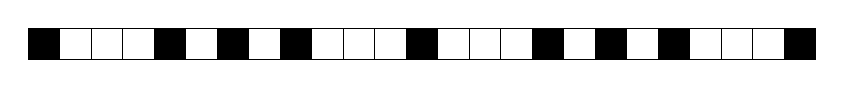
\begin{tikzpicture}
      \draw[step=4mm] (0,0) grid (10,.4);
      \fill%[pattern=north east lines]
        (0,0)   rectangle (.4,.4)  (1.6,0) rectangle (2,.4)
        (2.4,0) rectangle (2.8,.4) (3.2,0) rectangle (3.6,.4)
        (4.8,0) rectangle (5.2,.4)
        (6.4,0) rectangle (6.8,.4) (7.2,0) rectangle (7.6,.4)
        (8,0)   rectangle (8.4,.4) (9.6,0) rectangle (10,.4);
    \end{tikzpicture}
  \end{center}
  We can spot pretty quickly that this sequence is a palindrome.
  However, a far stronger geometrical relationship between the filled squares becomes evident when we present the same sequence as a two-dimensional grid.
  \begin{center}
    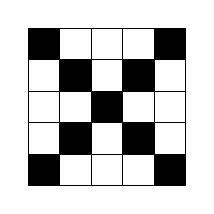
\begin{tikzpicture}
      \draw[step=4mm] (0,0) grid (2,2);
      \fill%[pattern=north east lines]
        (0,0)    rectangle (.4,.4)
                 rectangle (.8,.8)
                 rectangle (1.2,1.2)
                 rectangle (1.6,1.6)
                 rectangle (2,2)
        (2,0)    rectangle (1.6,.4)
                 rectangle (1.2,.8)
        (.8,1.2) rectangle (.4,1.6)
                 rectangle (0,2);
    \end{tikzpicture}
  \end{center}
  This goes to show that certain modes of presentation are preferred for certain patterns.
  Not all information is equally accessible in all modes of presentation.
\end{example}

For a more thorough treatment of informativeness, we need a formal description of what we mean by information.
Typically, we link information to \emph{entropy}~\parencite{cover2006elements}, thus bringing statistics on board the study of informativeness.
Information, then, relates to a property of a data source that expresses how unpredictable the data source is.
In other words, information is what breaks the mold, as it defies our expectation.

Different kinds of data come with different expectations.
Some patters are more clearly presented in certain modes of presentation, and conversely some modes of presentation make us expect certain patterns.
A musical idea, for example, is hard to convey in a painting, yet may be precisely what an audience member in a concert is listening for.
The medium is thus part of the message and information is context-dependent.

\begin{example}
\label{ex:pin}%
  \indexkey{example!distribution of PINs}%
  \pgfmathsetmacro{\numpasswords}{14830591}%
  Let us take a look at the distribution of passwords that are made up of four digits.
  Four-digit passwords are the de~facto norm for a personal identification number, a PIN.
  A naive analysis would be that when we have no information about someones PIN and we have to guess it, we stand a one in ten~thousand chance of being correct.
  As we shall see, this is far from the truth when the PIN was chosen freely by its owner.

  To estimate the distribution of PINs in use, we filter a collection of over half a billion passwords for four-digit passwords.
  The collection is made up of passwords obtained in data breaches and was put together by \textcite{hunt2018have}.
  This tactic was first employed by \textcite{berry2012pin} and our approach here is much the same as his.
  In the database we use, \num{\numpasswords} uses of a four-digit password are recorded.
  Based on the relative frequency of each PIN, we quickly find that they are not distributed uniformly.
  As can be seen in Figure~\ref{fig:pinprobability}, the bulk of the distribution of PINs can be approximated by a straight line in a log--log plot.
  Therefore, our PINs are an example of a dataset that adheres to Zipf's law.
  This empirical law states that the frequency of a word in a corpus of natural language is inversely proportional to its rank.
  Outside natural language, distributions of this kind have been observed in many real-world data encountered in the physical and social sciences \parencite{newman2005power}.
  \begin{figure}
    \centering
    \begin{tikzpicture}
      \begin{loglogaxis}[
        width=10cm,
        height=15cm, % Will be reduced automatically
        axis equal image=true,
        clip mode=individual,
        xlabel={rank},
        ylabel={empirical probability},
      ]
        \addplot [
          only marks,
          mark=+,
          scatter,
          scatter/use mapped color={draw=mapped color},
          point meta={max(1, min(10000, (55*\thisrowno{2}/\numpasswords)^(-1/0.7)))},
        ] table [
          header=false,
          x index=3,
          y expr={\thisrowno{2}/\numpasswords},
        ] {pwned.dat};
        \addplot [
          samples at={1, 10000},
        ] {x^(-0.7) / 55};
      \end{loglogaxis}
    \end{tikzpicture}
    \caption{
      A log--log plot of the empirical probability of PINs by rank, in decreasing order of likelihood.
      Except for one outlier on the top-end, the PIN~\code{1234}, and a thin tail of less than 5\% of the PINs, the distribution can be approximated by a power law.
      Points are colored in accordance with their rank as approximated by the fitted power law.
      Because the horizontal axis is logarithmic, the colormap appears distorted.
    }
    \label{fig:pinprobability}
  \end{figure}

  Having found that PINs are not distributed uniformly, we wonder what can be said about the specifics of their distribution.
  In Figure~\ref{fig:pinprobability}, we cannot see which PINs correspond to which data points.
  Therefore, we turn to a different plot, depicting the rank of all PINs as estimated by our approximation of the empirical probability distribution, Figure~\ref{fig:pinheatmap}.
  \begin{figure}
    \centering
    \begin{tikzpicture}
      \begin{axis}[
        x=1mm, y=1mm,
        enlargelimits=false,
        tick align=outside,
        xtick={10, 20, ..., 90},
        extra x ticks={0},
        extra x tick labels={$00$},
        ytick={10, 20, ..., 90},
        extra y ticks={0},
        extra y tick labels={$00$},
      ]
        \addplot [
          matrix plot*,
          point meta={max(1, min(10000, (55*\thisrowno{2}/\numpasswords)^(-1/0.7)))},
          mesh/cols=100,
        ] table [
          header=false,
        ] {pwned.dat};
      \end{axis}
    \end{tikzpicture}
    \caption{
      A heatmap of PINs, inspired by a similar heatmap created by \textcite{berry2012pin}.
      The first two digits of the PIN determine its horizontal position, while the last two digits determine the vertical position.
      This way, the PIN~\code{0099} ends up at the top-left corner and the PIN~\code{9900} ends up at the bottom-right corner.
      The colors are based on the clamped power law fitted on the bulk of the PINs in Figure~\ref{fig:pinprobability}.
      Darker colors represent more frequent occurrence of a PIN in the database.
      As witnessed by the area of light-colored PINs on the left side of the plot, many PINs in the tail of the distribution start with a~\code{0}.
    }
    \label{fig:pinheatmap}
  \end{figure}

  In Figure~\ref{fig:pinheatmap}, we can recognize many categories of PINs that occur frequently.
  Some of these categories are purely syntactical.
  The prominent diagonal line, for instance, represents PINs of the form \code{abab}.
  Algorithmic complexity theory is well-suited to deal with such patterns.
  We may therefore expect the universal distribution~\parencite{li2008introduction}, though uncomputable, to be a good model for the distribution of PINs.
  For this to be true, all structure in Figure~\ref{fig:pinheatmap} must be essentially syntactical.
  However, there is also a strong vertical line of PINs of the form \code{19ab}, continuing shortly into the \code{20ab} pattern.
  The prevalence of such PINs can easily be explained as people choosing a year as they PIN and most emotionally meaningful years being in the recent past.
  This explanation is not a syntactical one.
  Of course, a model for algorithmic complexity can include this contextual information at the cost of only an additive constant.
  With little more modeling of context, also the frequent occurrence of PINs formatted as dates, MMDD or DDMM, can be covered.
  Note that the lengths of the months generate a distinct and recognizable pattern in our heatmap.
  Yet, we claim that the additive constant relative to a standard abstract definition of Turing machines will have to become huge.
  Some properties of the plot in Figure~\ref{fig:pinheatmap} can easily be explained culturally, but lack any numerical meaning.
  For instance, the PIN~\code{5683} occurs particularly often, which can be explained by its meaning as a phoneword.
  A phoneword is a word spelled on a traditional phone keypad using ITU~E.161 assigned letters.
  The letters of the word \enquote{Love} are assigned the digits~\code{5683}, respectively.
  It is thus not reasonable to expect the distribution of PINs to approximate the universal distribution in any way.
  We are better off identifying as many meaningful categories of PINs and build our model of PINs from there.
\end{example}

We can try to model a multitude of contexts so that we can deal with the information in each of them.
In doing so, however, we should control the amount of detail with which we describe our models.
Surely, we do not want a taylor made model for every conceivable arrangement of data.
In such a setting, every data sample would have a context in which the sample contains no information.
This is known as \emph{overfitting}~\parencite{grunwald2007minimum}.
Algorithmic statistics addresses overfitting by taking into account the complexity of a description of a model.
Interestingly, there are data sets for which no \emph{simple} model is a decent fit.
There are complex models in relation to which these data sets contain disproportionately little information.
In relation to any simple model, the information in these data sets is considerably higher.
From this observation, it follows that the minimum model complexity required to achieve a decent fit is a nontrivial property of a data set.
Thus, a parameterized analysis of data sets, where the parameter is this minimum model complexity, emerges.

In traditional algorithmic statistics, Kolmogorov complexity is used in the assignment of complexity to models.
By doing so, it is possible to include practically all effective models in the analysis of informativeness.
As a result, the central probability distributions of interest in traditional algorithmic statistics is the universal distribution.
We have seen in Example~\ref{ex:pin} that the universal distribution is not always the best for a particular domain.
Fortunately, it is possible to employ the methods of algorithmic statistics in a setting where we restrict our attention to a specific collection of models.

\subsection{Computational Redundancy}


\section{Parameterized Complexity Theory}
\label{sec:parameterized_complexity_theory}%
